\title{A escala de decibel (dB) e suas derivações.}
\author{Lucas Francisco do Nascimento Santos}


\date{Junho 2022}

\begin{document}

\maketitle

\textbf{ Projeto Integrador (PI) – Professor: Eduardo Heredia }
\
\section{Resumo}
	O decibel que é representado pelo (dB) ele não é uma unidade de medida, não mede nada diretamente, ele é mais parecido com a porcentagem, então, a porcentagem ela estabelece uma relação entre duas grandezas, por exemplo: as vendas subiram 25 neste ano, então quer dizer que 25 é uma relação de um antes e um depois. Então ela estabelece uma relação entre duas grandezas iguais as vendas antes e as vendas depois, e a porcentagem faz uma relação, se ela aumentou,diminuiu quanto ela aumentou e quanto ela diminuiu.A idéia do decibel é mais ou menos a mesma idéia da porcentagem.
	Palavras chaves: Decibel e medida.
	\newline
	
	\begin{figure}[h]
    \centering
    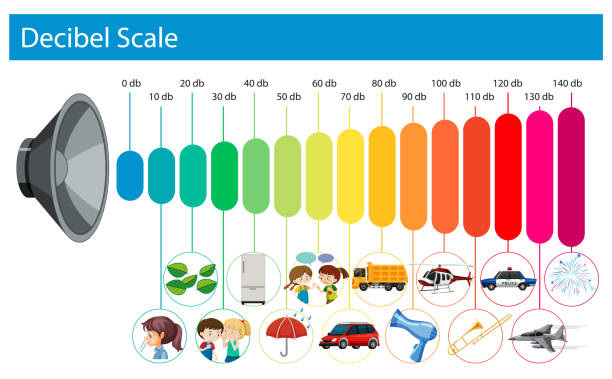
\includegraphics[width = 14cm]{istockphoto-1392255747-612x612.jpg}
    \label{fig:my_label}
    \end{figure}
	
	Fonte da imagem: https://www.facebook.com/djschoolmontreal/photos/C3A9chelle-des-niveaux-de-dC3A9cibel-rC3%A9f-httpswwwdiphoneventcomindexphple-bog11-les-ba/2628184493867411/
	
\section{Introdução}
    O decibel (dB), nos dias atuais é usado como uma comparação de valores de potência e tensão elétricas, desta forma, pegando dois valores de potência, pode informar esses dois valores e converter esse conjunto em decibel.
    A idéia do decibel surgiu na época das telecomunicações, por Alexander Graham Bel, ele com sua empresa de comunicações e telégrafos e depois mais atualmente a sua empresa de telefonia.
    Quando ele estava fazendo as linhas de telégrafos ele reparou que quando ele colocava um transmissor do telegrafo em um determinado ponto e fazia o cabeamento até o outro ponto, ele percebeu que o sinal chegava no destino dez vezes mais fraco, ou seja, o sinal que chegava era 0,1 do sinal que saia. E se ele pegasse desse segundo ponto e traçasse mais uma milha o sinal novamente caia 10 vezes. Inicialmente essa diminuição de dez vezes, Graham Bel chamou de 1TU, mas quando o Graham bel morreu , passaram chamar de 1bel em sua homenagem.
    Então o bel é nada mais que, um valor que é 10 vezes maior ou um valor 10 vezes menor que o valor informado.  
    \newline
    
    \begin{figure}[h]
    \centering
    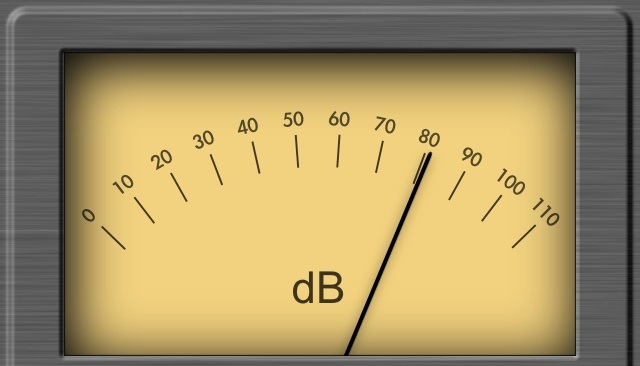
\includegraphics[width = 14cm]{imagem2.jpg}
    \label{fig:my_label}
    \end{figure}
     
    Fonte: https://residential-acoustics.com/decibel-levels-sometimes-negative/
    \newpage
    
    \section{Desenvolvimento}
	O decibel é uma representação em escala logarítmica de uma razão entre dois números.
    
    
    Para sinais de potência ou intensidade:
    
   \begin {equation}
   L_{dB} = 10.log_{10}(\frac{l}{ L_{0}})
   \end{equation}
    \newline
    
    Explicando a fórmula acima, o valor em dB ele vai ser 10 x log10 com o argumento do valor que queremos converter dividido pelo um valor de referência.
    \newline
    
    Convertendo um valor em dB para base decimal:
    \newline
    
     \begin {equation}
      L=L_{0}.10.(\frac{ldB}{ {10}})
      \end{equation}
      \newline
      
      Explicando a fórmula acima, basicamente temos que  inverter a equação, e isso vai resultar a fórmula citada acima.
Então o valor original vai ser igual ao sinal de referência, multiplicado por 10, (por que o logaritmo é na base 10), elevado o valor em dB e dividido por 10 também. Essa é a expressão da conversão reversa  de dB para uma base decimal.
Um detalhe importante, se o sinal que estiver analisando não  for um sinal de intensidade ou um sinal de potência, for por exemplo: um sinal de tensão, corrente ou  pressão sonora ,também informação de ganho que na prática uma razão entre essas grandezas a fórmula como calcula ou a forma como computa o dB muda para a formula  mostrada abaixo:
\newline

\begin {equation}
     V_{dB}=20.log_{10}(\frac{V}{ {V0}})
      \end{equation}
\newline   

Neste caso usamos o número 20 x log10 e não mais o número 10 x log na base 10. Toda vez que pegarmos o sinal e multiplicarmos  ele por 10, o que vai resultar em dB vou somar ao meu valor original de 20 dB.
È importante saber que quando tratamos com sinais de grandezas como tensão e corrente, a lógica da conta um pouco em relação aos sinais de intensidade de potência. 
Oque é dBV, dBU e dBM:
-Nada mais do que a definição do sinal de referência de uma conversão para decibel.
dBV – Um sinal de tensão que usa o V0 = 1V;
dBM – Um sinal de potência que usa I 0 = 1mW;
dBU – Um sinal de tensão que usa V 0 = 0,775V; ( Esse é o sinal necessário para produzir 0dBM  em uma carga).
Um detalhe a ser observado, se estiver definindo um valor em dB para um ganho que na prática é razão entre duas grandezas por exemplo: a tensão de saída (Av=vo/vi), como o argumento dessa conversão para dB já é a razão entre dois números não vai ter um sinal de referência, ou seja, vai fazer uma conversão direta do valor do ganho , por exemplo o valor do amplificador ganho é igual a 10, então o argumento da minha amplificação para dB é 10, então a conversão é mais direta não será preciso dividir o valor que queremos por um sinal de referência.
\newpage

\section{Coclusão}

Pode-se retomar o que foi apresentado na introdução e no desenvolvimento sobre a escala de decibel que é uma unidade derivada do bel, a  vantagem do decibel, é por ser uma escala logarítmica ela mostra sinais que estão muito próximos ou sinais que estão muito distantes de uma forma muito mais palpável para nos entendermos, isso é uma vantagem de uma escala não linear, podemos concluir  que o decibel é uma forma de comprimir a faixa de valores facilitando a leitura e operações matemáticas.
\newpage

\section{Referência}
\textbf{ESCALA DE DECIBEL. }.O que é decibel. \textbf{Disponível em: https://www.embarcados.com.br/o-que-e-decibel/ .} Acesso em: 15 Jun. 2021. Citado na página 1, 2 e 3.
\newline

\textbf{ESCALA DE DECIBEL. Decibéis. Disponível em: https://www.hear-it.org/pt/o-que-e-db-e-frequencia Acesso em:}Acesso em: 15  Jun. 2021. Citado na página 1, 2.
\newline

\textbf{ESCALA DE DECIBEL.}. Fórmula para calcular decibéis . \textbf{Disponível em : https://mundoeducacao.uol.com.br/matematica/medindo-intensidade-dos-sons.htm } Acesso em: 15 Jun. 2021. Citado na página 1, 2 e 3.
\newline

\textbf{ESCALA DE DECIBEL.}. Vantagens do decibel . \textbf{Disponível em: https://pt.wikipedia.org/wiki/Decibel}  Acesso em: 15  Jun. 2021. Citado na página 1, 2 e 3.

      
      

\end{document}